\chapter{Courant alternatif et électricité domestique}

\paragraph{Objectif}

\begin{enumerate}
  \item L'étudiante connaîtra la définition de courant alternatif, de tension
    et de courant effectif.
\end{enumerate}


\section{Courant alternatif}

\marginpar{Tremblay \S 12.1}

Le courant produit par une génératrice (dont nous parlerons un peu plus tard
dans le cours) est souvent un courant alternatif, c'est-à-dire qu'il circule
parfois dans une direction, parfois dans l'autre. Cette variation de courant
est causée par une tension alternative produite par la source. Le cas le plus
courant est celui d'une source qui produit une tension variant de manière
sinusoïdale :
\[
  \Delta V = \Delta V_0 \sin(\omega t + \phi)
\]
où $\Delta V_0$ représente la tension maximale (ou l'amplitude de la tension),
$\omega$ est la fréquence angulaire, $\phi$ est la constante de phase. En
Amérique du Nord, la fréquence est de $f = \SI{60}{Hz}$ ce qui correspond à une
fréquence angulaire de
\[
  \omega = 2 \pi f = \SI{377}{rad/s}
\]
Le courant produit par une telle tension varie aussi sinusoïdalement
\[
  i = i_0 \sin(\omega t + \phi')
\]
Dans le cas d'un simple circuit résistif, le courant et la tension sont en
phase ce qui signifie que $\phi' = \phi$. Pour simplifier la suite de cette
discussion, nous considérerons que la constante de phase vaut zéro. Dans ce
cas, la loi d'Ohm nous permet de déduire directement que
\[
  \Delta V = R i
\]
à tout moment. La puissance fournie à l'élément résistif est
\begin{align*}
  P &= \Delta V i  \\
    &= \Delta V_0 i_0 \sin^2 (\omega t) \\
    &= P_0 \sin^2 (\omega t)
\end{align*}

On remarque que la tension moyenne et le courant moyen sont tous les deux nuls,
mais que la puissance moyenne ne l'est pas (elle vaut $P_0 / 2$). Afin de
caractériser le courant par des quantités simples, on définit la
\textbf{tension effective} et le \textbf{courant effectif} comme étant les
valeurs de tension et de courant en courant continu qui produiraient la même
puissance moyenne. On a donc
\begin{align*}
  P_\mathrm{moy} &= \frac{1}{2} P_0  \\
  \Delta V_\mathrm{eff} &= \frac{1}{\sqrt{2}} \Delta V_0  \\
  i_\mathrm{eff} &= \frac{1}{\sqrt{2}} i_0  \\
\end{align*}
Lorsqu'on prend des mesures dans un circuit en courant alternatif, le
multimètre donne une lecture des valeurs effectives.

\begin{center}
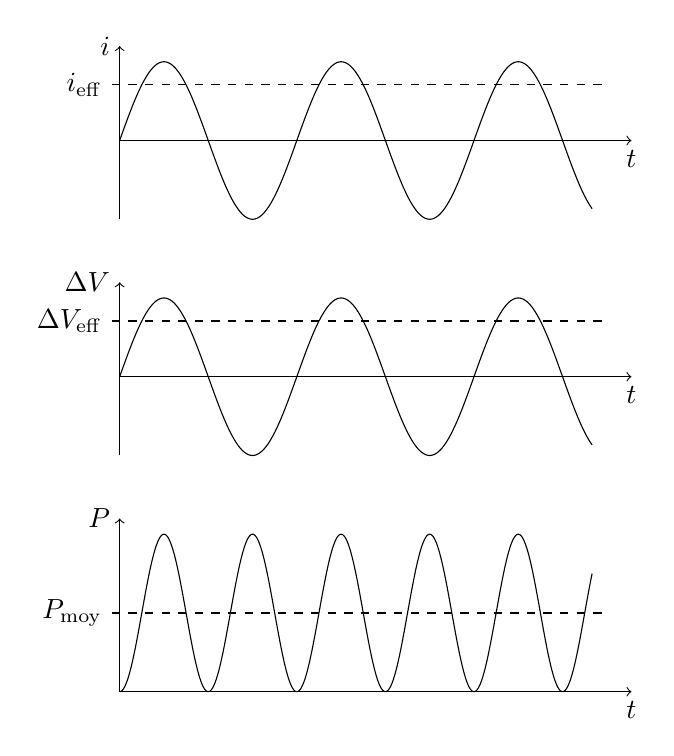
\begin{tikzpicture}
  \draw[->] (0, 6) -- (0, 8.2) node[left] {$i$};
  \draw[->] (0, 7) -- (6.5, 7) node[below] {$t$};
  \draw[domain=0:6, smooth, samples=500, variable=\t] plot ({\t}, {sin(160 * \t) + 7});
  \draw[dashed] (-0.1, 7 + 0.7071) node[left] {$i_\mathrm{eff}$} -- ++(6.3, 0);
  \draw[->] (0, 3) -- (0, 5.2) node[left] {$\Delta V$};
  \draw[->] (0, 4) -- (6.5, 4) node[below] {$t$};
  \draw[domain=0:6, smooth, samples=500, variable=\t] plot ({\t}, {sin(160 * \t) + 4});
  \draw[dashed] (-0.1, 4 + 0.7071) node[left] {$\Delta V_\mathrm{eff}$} -- ++(6.3, 0);
  \draw[->] (0, 0) -- (0, 2.2) node[left] {$P$};
  \draw[->] (0, 0) -- (6.5, 0) node[below] {$t$};
  \draw[domain=0:6, smooth, samples=500, variable=\t] plot ({\t}, {-cos(320 * \t) + 1});
  \draw[dashed] (-0.1, 1) node[left] {$P_\mathrm{moy}$} -- ++(6.3, 0);
\end{tikzpicture}
\end{center}

\subsection*{Exercice}

\marginpar{Diapo}

La plupart des circuits dans votre maison fonctionnent sur le \SI{120}{\volt}
(effectif).
\begin{itemize}
  \item Quelle est la valeur maximale de tension dans un tel circuit?
  \item Une bouilloire fonctionne avec un élément à \SI{900}{W}, quel est le
    courant effectif qui circule dans la bouilloire?
\end{itemize}

\begin{align*}
  \Delta V_0 &= \sqrt{2} \Delta V_\mathrm{eff} = \SI{169.7}{\volt} \\
  i_\mathrm{eff} &= P_\mathrm{moy} / \Delta V_\mathrm{eff} = \SI{7.50}{\ampere}
\end{align*}


\section{Électricité domestique}

\marginpar{Tremblay \S 12.8}

La maison est reliée au transformateur d'Hydro-Québec par trois fils : deux
sont à une tension alternative d'amplitude \SI{170}{V} et de fréquence
\SI{60}{Hz} mais avec une différence de phase de \SI{180}{\degree} (noir et
rouge), l'autre est
à un potentiel constant de \SI{0}{V} (blanc). Ces trois fils entrent dans
maison et dans le panneau électrique principal. Dans le panneau électrique
principal, le fil blanc est connecté à une mise à la terre qui est un fil de
cuivre de gros calibre relié au système d'aqueduc de la ville, c'est une mise à
la terre. Le fil noir alimente un des côtés du panneau électrique alors que
le fil rouge alimente l'autre côté.

\begin{center}
  \includegraphics[width=\textwidth]{09-courant-alternatif/figures/panneau.pdf}
\end{center}

Tous les circuits dans la maison sont reliés au panneau électrique principal en
parallèle. La plupart sont reliés au neutre et au fil rouge ou au fil noir de
telle sorte qu'ils sont connectés à une différence de potentiel effective
de \SI{120}{V}. Pour les appareils consommant plus d'électricité (comme le four
et la sécheuse), on crée un circuit connecté au fil rouge \textit{et} au fil
noir ce qui donne une tension effective de \SI{240}{V}.


\subsection*{Exercice}

Comment doit être connectée un ampoule à deux interrupteurs à trois voies?
\begin{center}
  \includegraphics[width=0.4\textwidth]{09-courant-alternatif/figures/ampoule-trois-voies.pdf}
\end{center}


\subsection*{Exercice}
On suppose qu'une prise de courant et une ampoule sont sur le même circuit.
L'ampoule est allumée. Quelqu'un branche un sèche-cheveu dans la prise de
courant et l'allume. Qu'arrive-t-il à l'intensité de la lumière émise par
l'ampoule?

Le sèche-cheveu nécessite beaucoup de puissance et donc un courant élevé
parcourera le fil entre la prise de courant et le panneau principal. Puisque le
fil a une certaine résistance électrique, la présence de ce courant élevé
causera une chute de potentiel dans le fil et l'ampoule ne sera plus connectée
à une tension effective de \SI{120}{V} mais à une tension plus faible. Par
conséquent, le courant traversant l'ampoule et donc son intensité diminueront.



